\subsect{Sprint 6}{sprint6}

\underline{Fecha de inicio}: 11/11/2022

\underline{Fecha de fin}: 11/12/2022

\underline{Objetivo}:
Mejora de la observabilidad del sistema.

\underline{Descripción}:
En este sprint se pretende mejorar la observabilidad del sistema utilizando paneles para su administración.\ Estos
paneles se utilizarán para monitorizar el estado del sistema y para visualizar los datos de los logs obtenidos.
Todo esto conlleva la creación de 3 contenedores Docker adicionales:

\begin{itemize}
	\item Prometheus:
	Sistema de monitorización y alertas.
	\item Grafana:
	Sistema de visualización de datos.
	\item Loki:
	Sistema de logs.
\end{itemize}

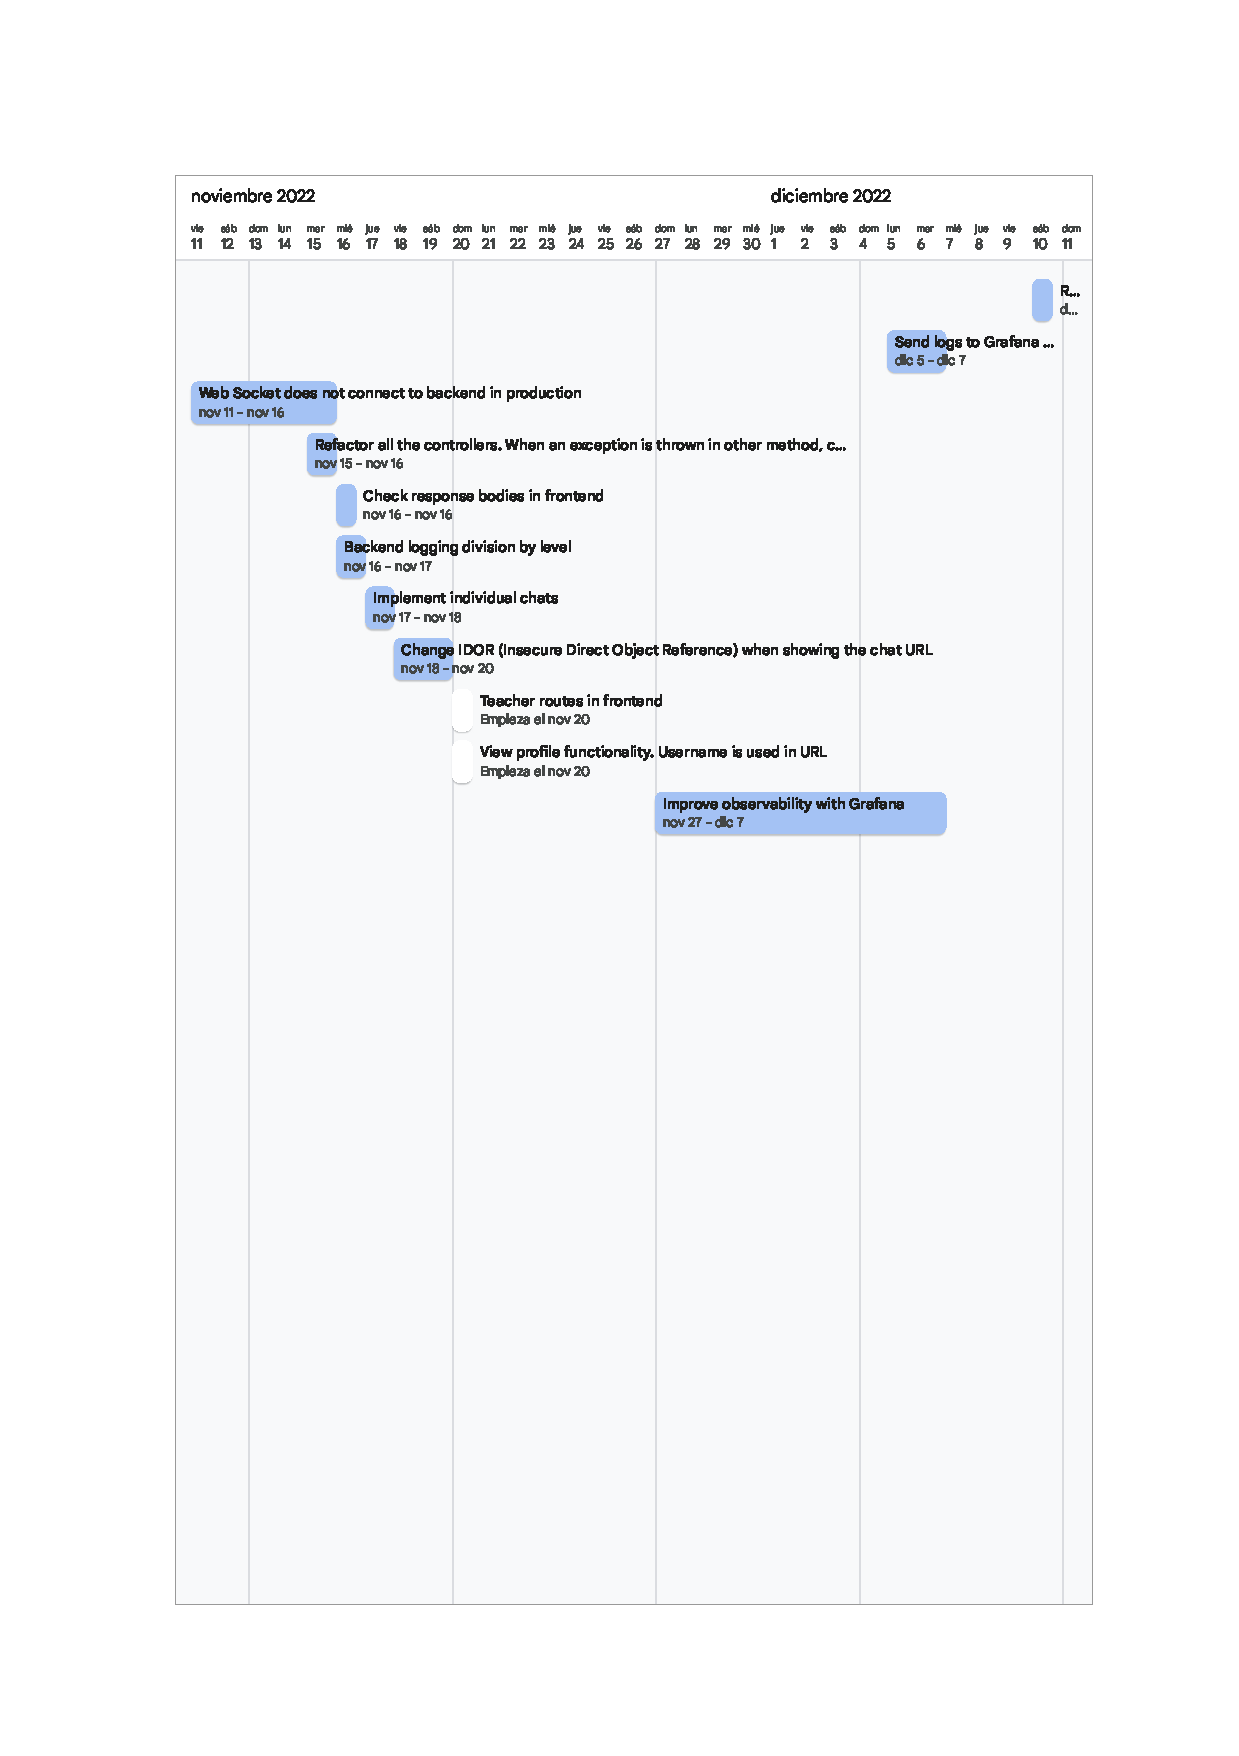
\includepdf[pages=-]{backlog/sprints/Sprint6.pdf}
